\begin{document}

%----------------------------------------------------------------------------------------
%       TITLE PAGE AND OUTLINE
%----------------------------------------------------------------------------------------
\title[Снижение задержки декодирования]{Методы снижения } % The short title appears at the bottom of every slide, the full title is only on the title page
\author{Н.В. Якуба} % Your name
\institute[СПбПУ] % Your institution as it will appear on the bottom of every slide, may be shorthand to save space
{
  Санкт-Петербургский Политехнический Университет Петра Великого \\ % Your institution for the title page
}
\date{14 июня 2018} % Date, can be changed to a custom date

\begingroup 
    \setbeamertemplate{headline}{}
    \begin{frame}
      %% \titlepage % Print the title page as the first slide
      \centering
      Санкт-Петербургский Политехнический Университет Петра Великого \\ % Your institution for the title page
      Высшая школа программной инженерии\\
      \vspace{0.1\textheight}
      \begin{block}{}
        \centering
        \Large{Методы снижения задержки при декодировании полярных подкодов}
      \end{block}
      \vspace{0.05\textheight}
      \begin{tabular}{lll}
        &\hspace*{0.25\textwidth}&\\
        Выполнил\\ студент гр. 23547/1 && Н.В. Якуба\\
        Руководитель\\ к.т.н., доцент && П.В. Трифонов\\
      \end{tabular}
      \vfill
      Санкт-Петербург\\
      2018
    \end{frame}
\endgroup

\begingroup 
    \setbeamertemplate{headline}{}
    \addtobeamertemplate{frametitle}{\vspace*{-\headheight}}{}
    \begin{frame}{Outline}
      % Table of contents slide, comment this block out to remove it
      \tableofcontents % Throughout your presentation, if you choose to use \section{} and \subsection{} commands, these will automatically be printed on this slide as an overview of your presentation
    \end{frame}
\endgroup

%----------------------------------------------------------------------------------------
%       PRESENTATION SLIDES
%----------------------------------------------------------------------------------------
\section{Early termination schemes}

\begin{frame}{Early Termination Approaches}
  \begin{columns}[t] % "c" - centered vertical alignment, "t" -- top vertical alignment
    \column{.47\textwidth} % Left column
    \textbf{Path metric based}
    \begin{itemize}
    \item Does not affect code parameters
    \item Sufficient performance gain can be reached
    \item Depend on channel $E_s/N_0$
    \item Unreliable due to equalization errors
    \end{itemize}

    \column{.47\textwidth} % Right column
    \textbf{Parity check based}
    \begin{itemize}
    \item Require additional bits to transmit
    \item Almost independent on channel $E_s/N_0$
    \item Can guarantee low false alarm probability
    \end{itemize}
  \end{columns}
\end{frame}

%----------------------------------------------------------------------------------------
% May be problems with \end{frame} in verbatim. Search StackOverflow.
\begin{frame}[fragile] % Need to use the fragile option when verbatim is used in the slide
\frametitle{Verbatim}
\begin{example}[Theorem Slide Code]
\begin{verbatim}

\begin{frame}
\frametitle{Theorem}
\begin{theorem}[Очень важная теорема]
$E = mc^2$
\end{theorem}

\end{verbatim}
\end{example}
\end{frame}

%----------------------------------------------------------------------------------------
\begin{frame}{Multiple Columns}
\begin{columns}[c] % The "c" option specifies centered vertical alignment while the "t" option is used for top vertical alignment

\column{.45\textwidth} % Left column and width
\textbf{Heading}
\begin{enumerate}
\item Statement
\item Explanation
\item Example
\end{enumerate}

\column{.5\textwidth} % Right column and width
Lorem ipsum dolor sit amet, consectetur adipiscing elit. Integer lectus nisl, ultricies in feugiat rutrum, porttitor sit amet augue. Aliquam ut tortor mauris. Sed volutpat ante purus, quis accumsan dolor.

\end{columns}
\end{frame}

%----------------------------------------------------------------------------------------
\begin{frame}{References}
\footnotesize{
\begin{thebibliography}{99} % Beamer does not support BibTeX so references must be inserted manually as below
\bibitem[Smith, 2012]{p1} John Smith (2012)
\newblock Title of the publication
\newblock \emph{Journal Name} 12(3), 45 -- 678.
\end{thebibliography}
}
\end{frame}

%----------------------------------------------------------------------------------------
\begin{frame}{DCRC and PC-CRC Schemes Comparison \#2}
  \begin{figure}
    \centering
    \includegraphics[width=0.7\linewidth]{plots/eps/{96}{40}_normal.eps}
    \captionof{figure}{Correct codeword transmission, $10^6$ iterations, $(96, 40)$ code, $L = 8$, $J = 23$, $J_{PC} = 4$, $a = 3$}
    \label{figure:dfcrc4_normal_96}
  \end{figure}
\end{frame}

%----------------------------------------------------------------------------------------
\begin{frame}{Blind structure}
  \begin{figure}
    \centering
    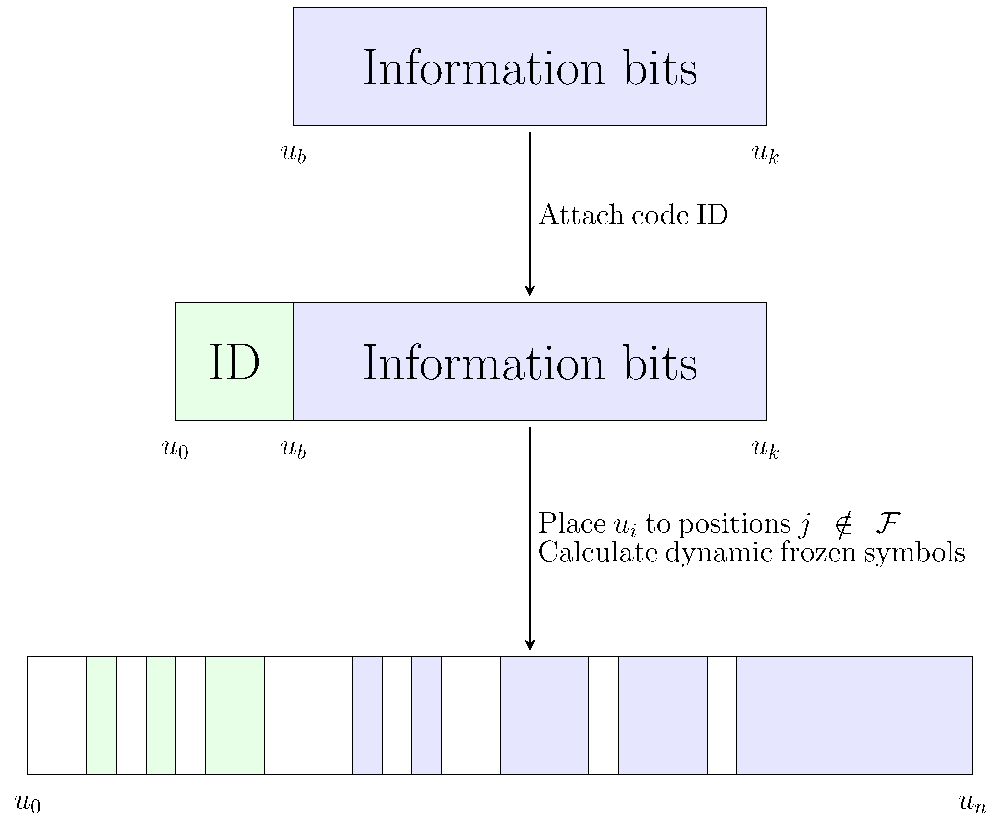
\includegraphics[width=0.7\linewidth]{pictures/BlindStructure.eps}
  \end{figure}
\end{frame}

%----------------------------------------------------------------------------------------
\begin{frame}{Сложность и задержка декодирования}
  \begin{table}
    \caption{Сложность декодирования $(1536, 768)$ кода, число операций}
    \begin{tabular}[c]{|l|ll|ll|}
      \hline
      & \multicolumn{2}{l|}{Сложения} & \multicolumn{2}{l|}{Сравнения}\\
      \hline
      $L$ & $A_m \otimes R_3$ & $A_{m'}$ & $A_m \otimes R_3$ & $A_{m'}$\\
      \hline
      1 & 3.5e+04 & 1.1e+04 & 2.1e+04 & 1.2e+04\\
      4 & 6.7e+04 & 4.2e+04 & 3.9e+04 & 5.0e+04\\
      8 & 9.8e+04 & 8.3e+04 & 5.5e+04 & 1.2e+05\\
      \hline
    \end{tabular}
  \end{table}

  Задержка декодирования $(1536, 768)$ кода предложенным списочным алгоритмом может быть уменьшена в $\approx 3$ раза по сравнению с классическим списочным алгоритмом декодирования полярных кодов
\end{frame}

%----------------------------------------------------------------------------------------
\begin{frame}{Summary}
  \begin{enumerate}
  \item PC based early termination scheme shows lower expected early termination phase than DCRC and Split-CRC schemes
  \item PC based scheme requires configuration of parameters depending on code used by the decoder
  \item DCRC scheme demonstrates the lowest FAR performance among all considered early termination schemes
  \item Additional parity checks can be used jointly with other early termination criterias to further lower expected early termination phase
  \end{enumerate}
\end{frame}

%----------------------------------------------------------------------------------------
\end{document} 
